\section{Bagian V --- Kompilasi Lima Visualisasi Komparatif Utama}
Figur 3 telah disajikan pada Bagian III (Gambar~\ref{fig:mlp}). Seluruh figur dibuat dari Test Set dan sampel ber-seed tetap.

\begin{figure}[H]
\centering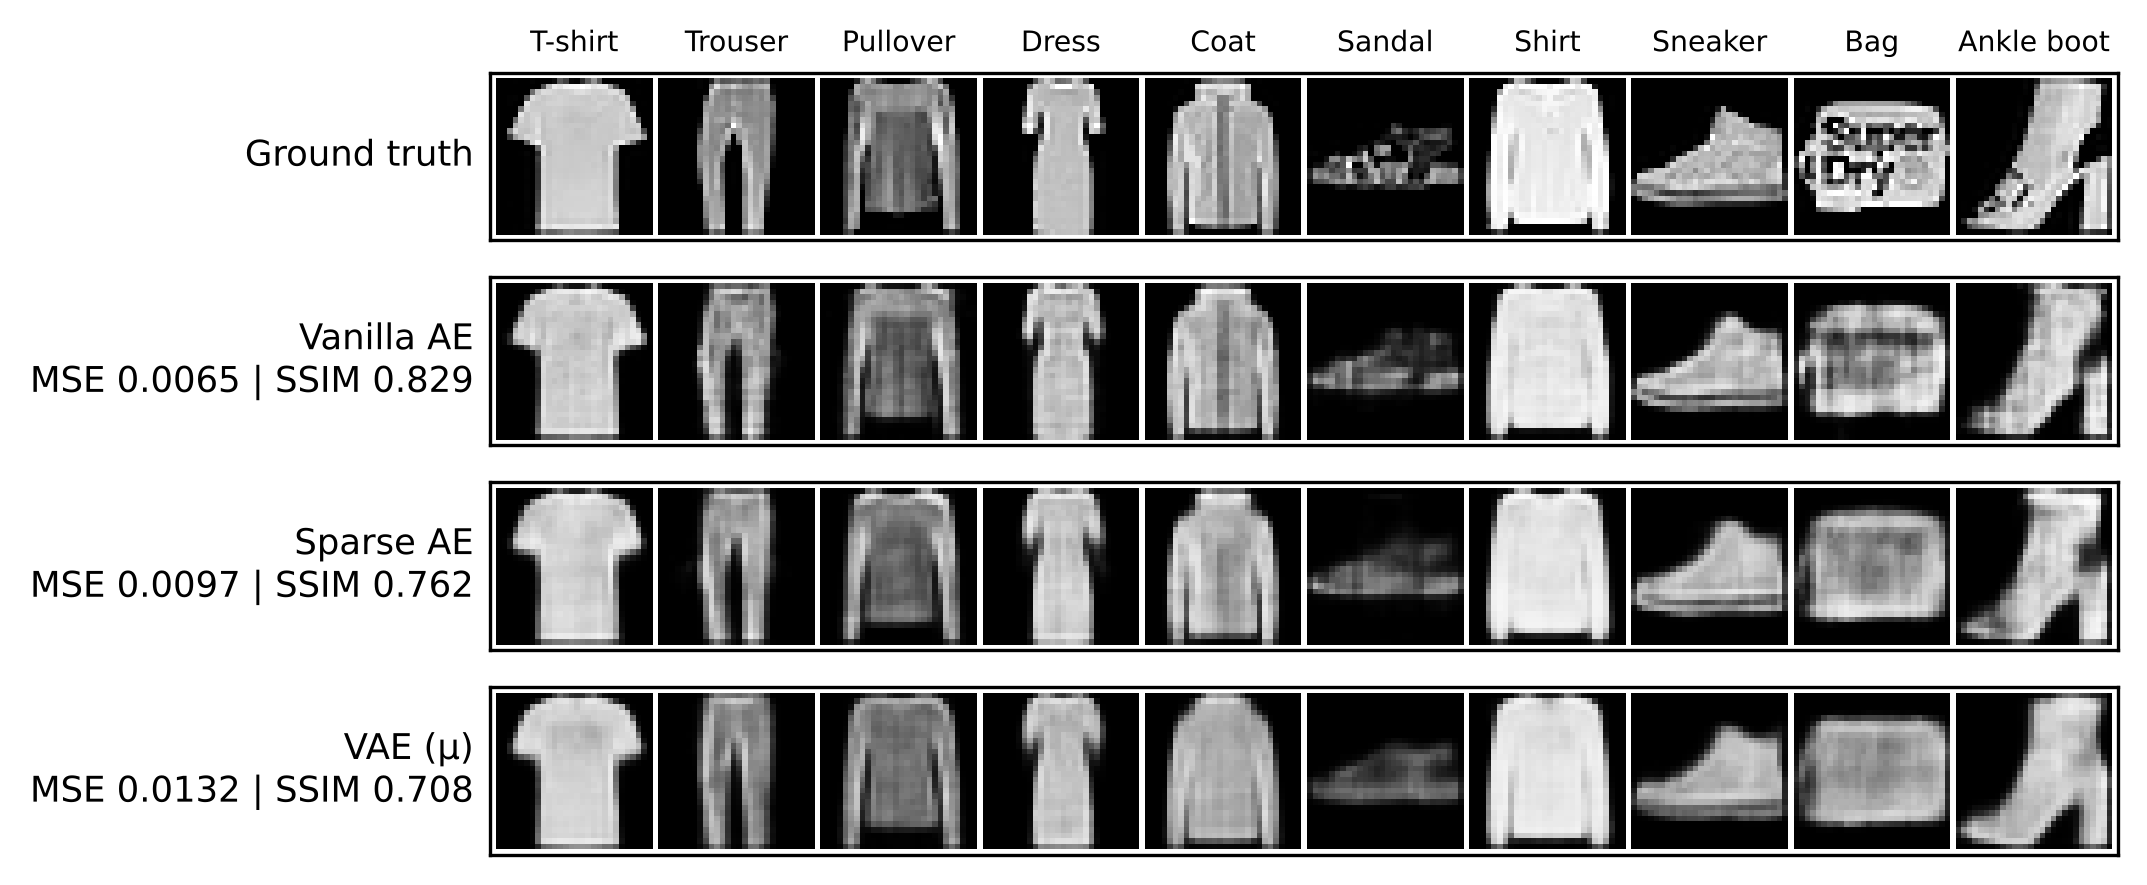
\includegraphics[width=0.95\linewidth]{../outputs/figures/fig1_rekonstruksi.png}
\caption{\textbf{Figur 1.} Rekonstruksi side-by-side satu citra test per kelas (kiri ke kanan: T-shirt $\to$ Ankle boot).
Baris: ground truth, Vanilla AE, Sparse AE, VAE (decode $\mu$).}
\label{fig:recon}
\end{figure}

\textbf{Analisis Figur 1.} Ketiga model mempertahankan siluet global, tetapi berbeda pada detail frekuensi tinggi.
Vanilla AE (kode padat, semua 64 unit aktif) paling banyak mempertahankan pola lokal---garis tali sandal, motif kaos,
dan tepi sepatu---sehingga SSIM-nya tertinggi (\SSIMAE). Sparse AE hanya mengaktifkan $\approx$\ACTSAE\ unit per citra:
kode berperilaku seperti kombinasi sedikit ``bagian'' (\emph{parts}) sehingga motif halus diganti tekstur generik dan
tepi sedikit melunak (SSIM \SSIMSAE). VAE paling buram (SSIM \SSIMVAE): selain loss piksel, suku KL memaksa posterior
$q(z|x)$ tiap citra melebar dan saling tumpang tindih, sehingga decoder belajar mengeluarkan rata-rata dari beberapa citra
yang berbagi wilayah laten yang sama. Detail seperti tulisan pada tas dan pola kotak-kotak hilang paling dulu.

\begin{figure}[H]
\centering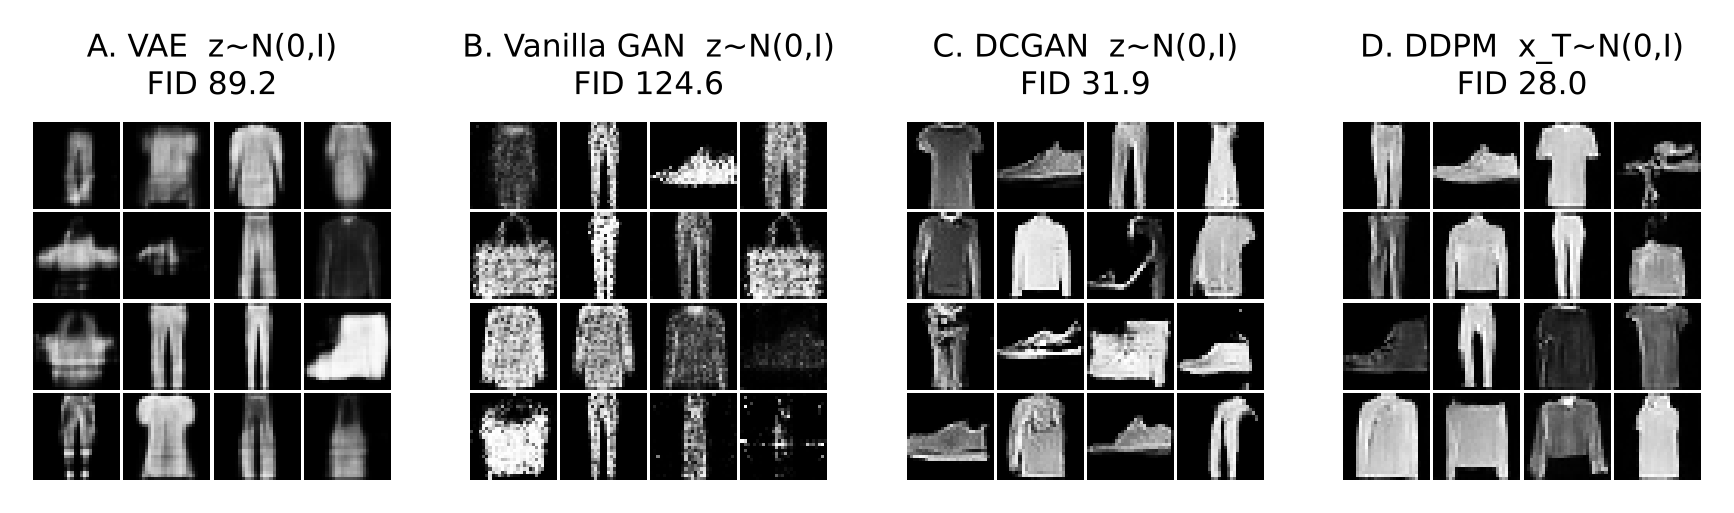
\includegraphics[width=\linewidth]{../outputs/figures/fig2_sampling.png}
\caption{\textbf{Figur 2.} Random generative sampling 4$\times$4 dari prior $\mathcal{N}(0,I)$: (A) VAE, (B) Vanilla GAN,
(C) DCGAN, (D) DDPM (reverse diffusion 1000 langkah dari $x_T\sim\mathcal{N}(0,I)$). Angka = FID (2.000 sampel).}
\label{fig:samples}
\end{figure}

\textbf{Analisis Figur 2.} \FigTwoText

\begin{figure}[H]
\centering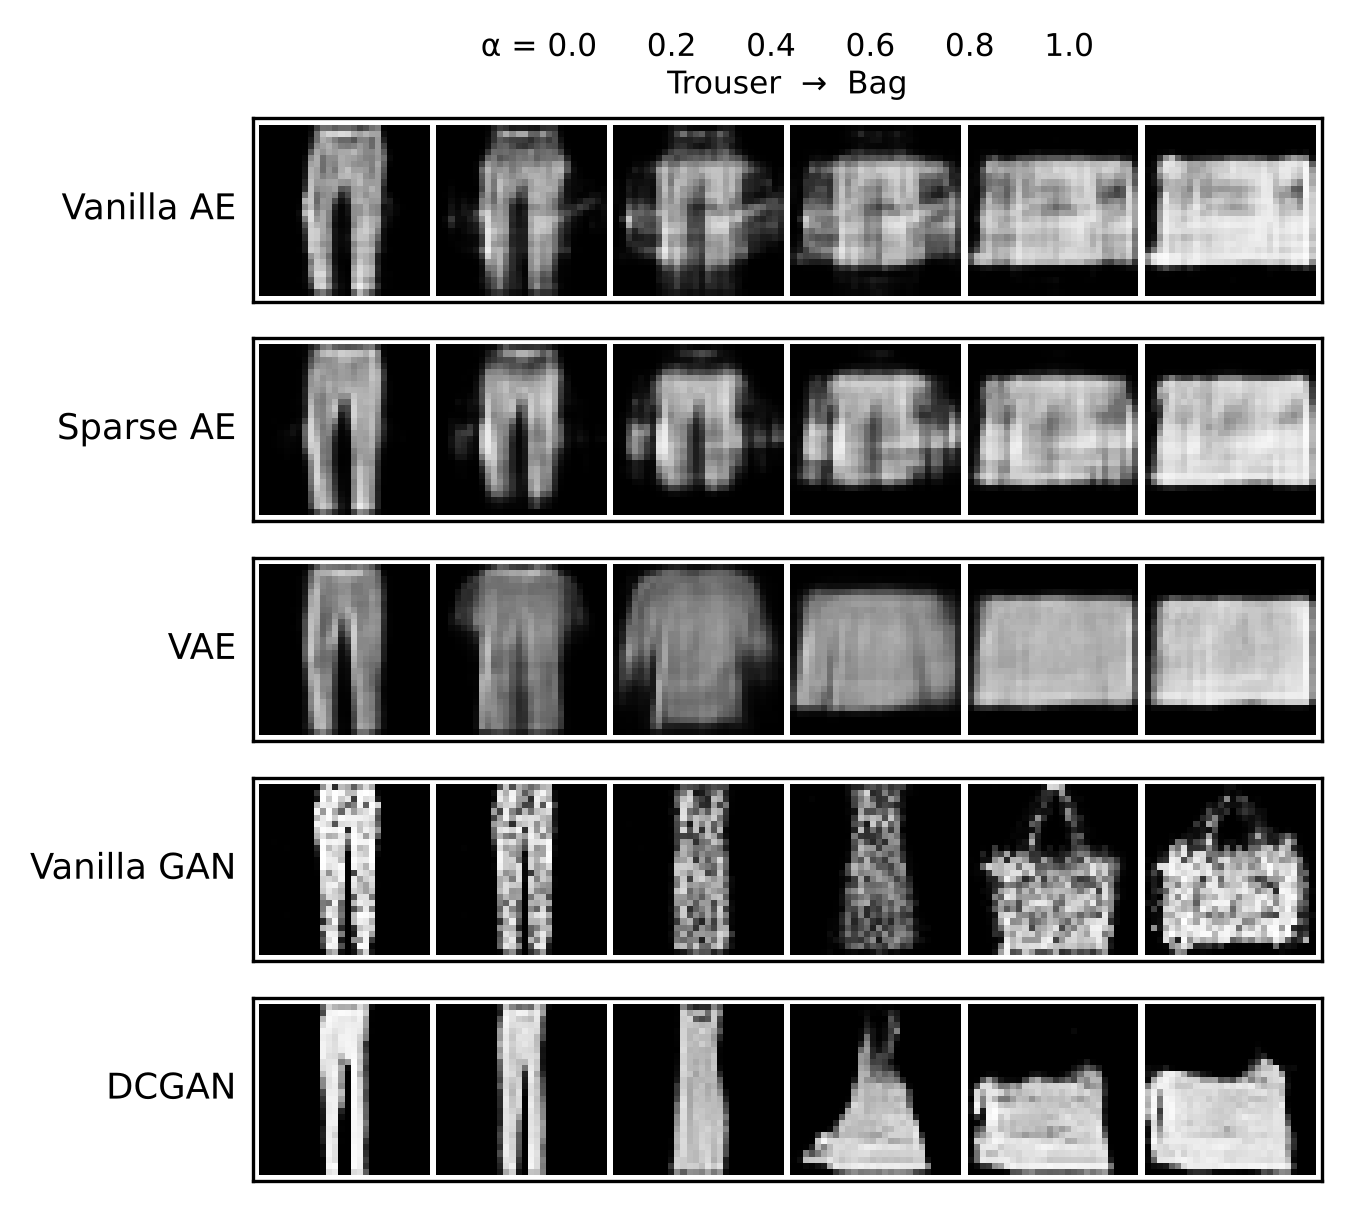
\includegraphics[width=0.66\linewidth]{../outputs/figures/fig4_interpolasi.png}
\caption{\textbf{Figur 4.} Interpolasi laten linier $z(\alpha)=(1-\alpha)z_A+\alpha z_B$ dari Trouser ke Bag.
AE/Sparse AE/VAE: $z_A,z_B$ = kode encoder dua citra test (VAE memakai $\mu$). GAN/DCGAN tidak memiliki encoder,
sehingga $z_A,z_B$ dipilih dari 5.000 vektor prior acak yang hasilnya diklasifikasikan MLP sebagai Trouser/Bag dengan
probabilitas tertinggi (keduanya $\approx$1,0).}
\label{fig:interp}
\end{figure}

\textbf{Analisis Figur 4.} Pada Vanilla AE dan Sparse AE, titik tengah ($\alpha=0{,}4$--$0{,}6$) berupa \emph{superposisi}
dua siluet---kaki celana tampak ``menembus'' badan tas, disertai pita-pita horizontal dan bercak kotak. Ini bukan objek
yang valid. Jarak titik tengah ke kode training terdekat (dinormalisasi terhadap kode test riil) mencapai
\VOIDAE$\times$ untuk Vanilla AE dan \VOIDSAE$\times$ untuk Sparse AE: lintasan lurus melewati wilayah laten yang
tidak pernah dilihat decoder. VAE berperilaku lain: transisinya halus dan setiap titik antara adalah pakaian yang masuk akal
(celana $\to$ atasan berlengan $\to$ tas), dengan rasio jarak terkecil (\VOIDVAE$\times$). Suku KL menarik seluruh posterior
ke dekat $\mathcal{N}(0,I)$ sehingga wilayah di antara dua kode terisi oleh posterior citra lain. GAN dan DCGAN juga
menghasilkan transisi semantik (celana $\to$ dress $\to$ tas) karena generator dilatih memetakan \emph{seluruh} massa prior
ke citra realistis; perbedaannya, Vanilla GAN tetap membawa derau bintik di setiap frame, sedangkan DCGAN bersih.

\begin{figure}[H]
\centering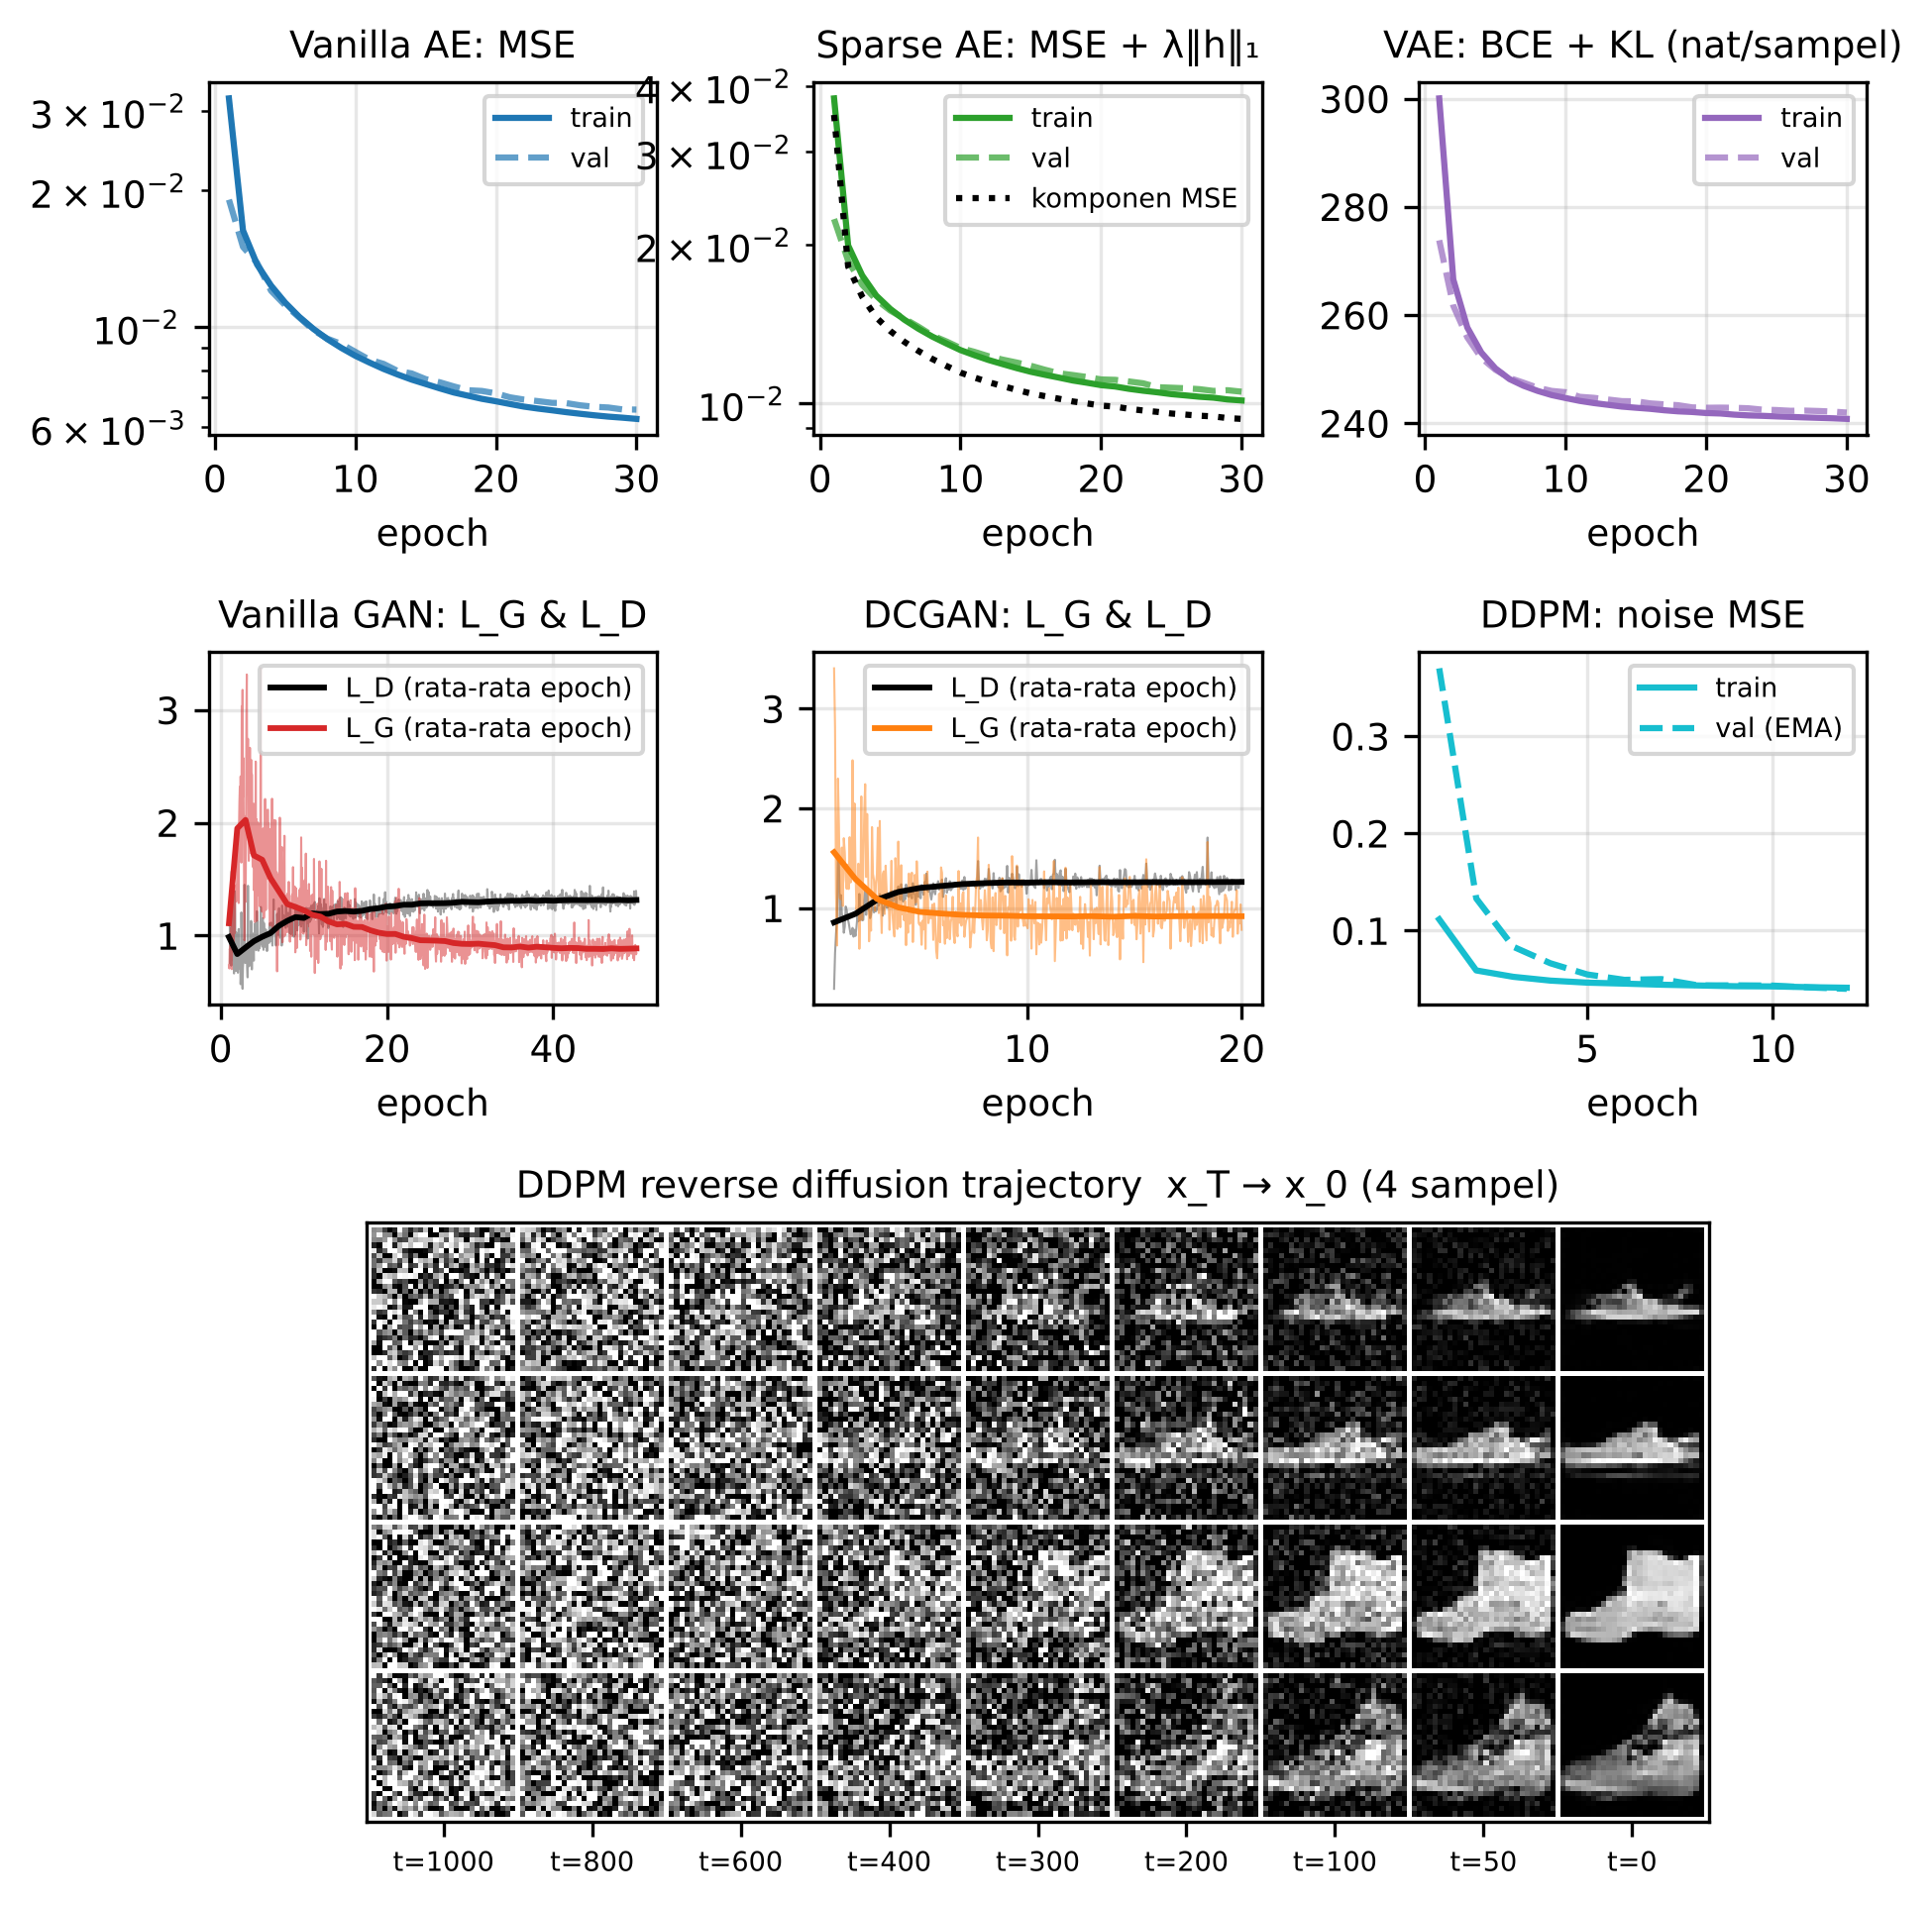
\includegraphics[width=\linewidth]{../outputs/figures/fig5_loss_ddpm.png}
\caption{\textbf{Figur 5.} Atas: kurva loss AE (MSE), Sparse AE (total dan komponen MSE), VAE (negatif ELBO, nat/sampel).
Tengah: loss $G$ dan $D$ Vanilla GAN dan DCGAN (garis tipis = setiap 20 iterasi, tebal = rata-rata epoch) serta noise-prediction
loss DDPM. Bawah: trajektori reverse diffusion DDPM $x_T\to x_0$.}
\label{fig:loss}
\end{figure}

\textbf{Analisis Figur 5.} Ketiga autoencoder turun monoton dengan selisih train--val kecil (Vanilla AE akhir: train
\AEtrain, val \AEval). Pada Sparse AE, komponen MSE turun lebih lambat daripada AE karena sebagian gradien dipakai untuk
menekan $\lVert h\rVert_1$. Kedua GAN tidak pernah ``konvergen'' dalam arti loss menuju nol: $\mathcal{L}_D$ naik
mendekati $2\log 2\approx1{,}39$ dan $\mathcal{L}_G$ turun mendekati $\log 2\approx0{,}69$, yaitu kondisi
$D(x)\approx D(G(z))\approx0{,}5$ (akhir Vanilla GAN: $D(x)=\DRGAN$, $D(G(z))=\DFGAN$; DCGAN: \DRDCGAN/\DFDCGAN).
Fluktuasi $\mathcal{L}_G$ per iterasi pada paruh akhir training lebih besar pada DCGAN (std \GSTDDCGAN) daripada Vanilla GAN
(std \GSTDGAN). DDPM turun mulus dari \DDPMfirst\ ke \DDPMlast\ (val EMA \DDPMval) tanpa osilasi. Trajektori bawah
memperlihatkan siluet kasar muncul pertama kali sekitar $t\approx300$--$200$ dan detail tekstur terbentuk pada $t<100$:
proses generasi berlangsung dari frekuensi rendah ke tinggi (\emph{coarse-to-fine}).
